\documentclass[12pt]{article}
%
\usepackage{graphicx}
\usepackage[margin=1in,footskip=0.2in]{geometry}%big footskip brings number down, small footskip br
\usepackage{amsmath}
\usepackage{amssymb}
\usepackage[T1]{fontenc}
\usepackage{listings}
\usepackage{bm}
\usepackage{hyperref}
\usepackage{setspace}
\usepackage[usenames]{color}
\usepackage[utf8]{inputenc}
\usepackage{wrapfig}
\usepackage{relsize}
\usepackage{psfrag}
\usepackage{dsfont}

%
%
\usepackage{titlesec}
\titlespacing*{\section}{0pt}{0.25\baselineskip}{0.25\baselineskip}
\titlespacing*{\subsection}{0pt}{0.5\baselineskip}{0.5\baselineskip}
%\titleformat*{\section}{\LARGE \bfseries}
\titleformat*{\section}{\large \bfseries}

%
\begin{document}

%
%

%
\pagenumbering{gobble}
\noindent
%NOAA Information Technology Incubator Proposal\\
\begin{centering}
NOAA INFORMATION TECHNOLOGY INCUBATOR PROPOSAL
\\$~$\\$~$\\$~$\\
for
\\$~$\\$~$\\$~$\\
{\bf IMPROVING CATCH ESTIMATION METHODS IN SPARSELY SAMPLED, MIXED-STOCK FISHERIES VIA HIGH PERFORMANCE COMPUTING.}
\\$~$\\$~$\\$~$\\$~$\\
11 April 2017\\
\end{centering}
$~$\\$~$\\$~$\\$~$\\$~$\\$~$\\$~$\\$~$\\$~$\\$~$\\
Total Budget: \$47,183
\\$~$\\$~$\\
Proposed Period: 1 October 2017 - 30 March 2018
\\$~$\\$~$\\
\noindent
Principle Investigator: Edward Dick$^\text{a}$ - edward.dick@noaa.gov\\
Co-Investigators: Nicholas Grunloh$^\text{b}$, Don Pearson$^\text{a}$, John Field$^\text{a}$, Marc Mangel$^\text{b,c}$\\
\\$~$\\$~$\\
$^\text{a}$ Fisheries Ecology Division, Southwest Fisheries Science Center, National Marine Fisheries Service, National Oceanographic and Atmospheric Administration, 110 McAllister Way, Santa Cruz, CA 95060, USA.\\
$^\text{b}$ Center for Stock Assessment Research, University of California, Santa Cruz, Mail Stop SOE-2, Santa Cruz, CA 95064, USA.\\
$^\text{c}$ Department of Applied Mathematics and Statistics, Jack Baskin School of Engineering, University of California, Santa Cruz, Mail Stop SOE-2, Santa Cruz, CA 95064, USA.

\clearpage
\pagenumbering{arabic}

%
%

%\begin{abstract}
\section{Abstract}
%
\underline{Description of proposed work:} 
Effective management of exploited fish populations, requires accurate estimates
of commercial fisheries catches to inform monitoring and
assessment efforts. In California, the high degree of heterogeneity in
the species composition of many groundfish fisheries, particularly those
targeting rockfish (genus $Sebastes$), leads to challenges in sampling all
potential strata, or species, adequately. Limited resources and
increasingly complex stratification of the sampling system inevitably
leads to gaps in sample data. In the presence of sampling gaps, ad-hoc
species composition point estimation is currently obtained according to
historically derived ``data borrowing'' (imputation) protocols which do not allow for
uncertainty estimation or forecasting. In order to move from the current
ad-hoc ``data-borrowing'' point estimators, we have
constructed Bayesian hierarchical models to estimate species
compositions, complete with accurate measures of uncertainty, as well as
theoretically sound out-of-sample predictions. Furthermore, we introduce
a computational method for discovering consistent ``borrowing''
strategies across over-stratified data. Our modeling approach, along with
a computationally robust system of inference and model exploration,
allows us to start to understand the effect of the highly stratified,
and sparse, sampling system on the kinds of inference possible, while
simultaneously making the most from the available data.
Our computational approach to model exploration is easily parallelized, but requires computing resources beyond our laboratory's current capabilities.
Adequate exploration of the plausible model space will require additional resources to produce results in a timeframe that is useful to managers and NOAA Fisheries scientists.
%\end{abstract}

%
\underline{RFP themes being evaluated:}
This proposal addresses a critical component of NOAA
Fisheries’ Stock Assessment Enterprise (\href{http://www.st.nmfs.noaa.gov/stock-assessment/}{http://www.st.nmfs.noaa.gov/stock-assessment/}), 
providing estimates of commercial catch to inform science-based
management of Federally-managed fish species, or stocks. As a fisheries application, the
proposed work falls under the “Non-Traditional Uses” category defined in the HPCC IT
Incubator RFP. Additionally, our proposed research is consistent with the “Data Analytics”
theme in that it creates a novel framework for analysis, discovery, and inference about an
indispensable input (catch) to modern stock assessment models.

%

%
\section{Significance}\label{significance}
%
\begin{figure}[h!]
	\centering
	%\vspace{-1cm}
	\begin{minipage}[c]{0.76\textwidth}
		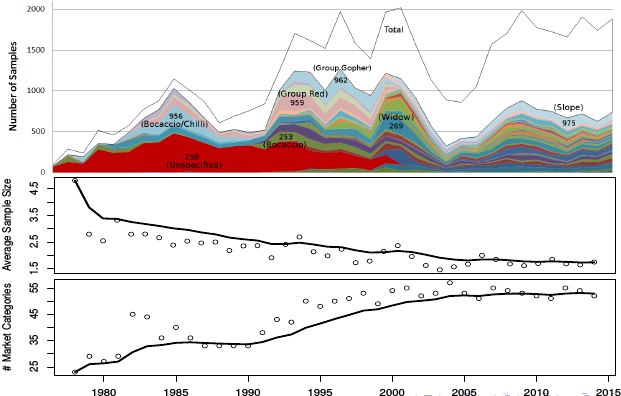
\includegraphics[width=0.98\textwidth]{sampleComplex.png}
	\end{minipage}\hfill
	\begin{minipage}[c]{0.24\textwidth}
		\caption{
		The $top$ $panel$ shows the total number of samples, from 1978 to 2015, in the major groundfish market categories.
		The $middle$ $panel$ shows the average sample size, per statum, decreasing through time, as the number of market categories increases, over the same period, in the $bottom$ $panel$.
		}
	\end{minipage}
%\color{red} Add proper caption. Strata more complex. Data more sparse. }
\end{figure}

%
In order to understand how fish populations respond to fishing, it is critical to obtain accurate estimates of how many fish are removed from the ocean (catch) and to quantify the precision of those estimates. 
Traditionally, population dynamics models used to measure this response to fishing (“stock assessments”) are conditioned on a time series of annual catches. 
These catch estimates are often treated as being known without error, despite the fact that they are derived from sampling programs that estimate the proportion of different species found within multiple sampling strata. 
Sampling error introduces uncertainty into estimates of the catch, and unsampled strata must be “filled in” through a process sometimes referred to on the U.S. West Coast as “borrowing” (i.e. data imputation). 
Historically, methods used to “borrow” information among strata have been ad-hoc in nature and driven by expert opinion of local managers (Sen et al. 1984, 1986) (Pearson and Erwin 1997). 
We seek to improve upon this practice through development of a model-based approach that provides estimates of catch and associated uncertainty, as well as an objective, defensible framework for model selection and data imputation.
Although the theoretical basis for a model based estimation of species composition in mixed stock fisheries has been advanced (Shelton et al., 2012), it has not yet been implemented successfully using actual historical or contemporary data.

%
The difficulties associated with the existing ad-hoc approach are magnified by an increase in the number of sampling strata over time, specifically the number of “market categories,” into which fishermen and dealers sort their catch (Figure 1, Bottom). 
The increase in the number of market categories (sampling strata) has not been matched by increases in sampling effort, resulting in a decline in the average number of samples per stratum (Figure 1, Middle). 
In other words, data are becoming more sparse, increasing our uncertainty in estimates of catch. 
Since the data are also stratified over a number of ports, fishing gear types, years, and quarters, inference is not possible without some sort of stratum pooling. 
Rather than rely so heavily on the previous, ad-hoc pooling rules which change based on the availability of samples, we hope to standardize any necessary pooling through an exhaustive search of the space (possible configurations) of pooled models. 
Pooling (and partial pooling) among strata is achieved using Bayesian hierarchical statistical models and model averaging (Gelman et al., 2014).

%
The proposed research will provide NOAA stock assessment scientists with a database of model-based catch estimates and associated estimates of uncertainty for California’s commercial rockfish fisheries going back several decades. 
Quantifying and propagating uncertainty in catches is critical to NOAA’s efforts to provide meaningful and transparent science advice to fisheries managers. 
Funds awarded through this RFP will overcome the limitations of our available computational servers, allowing us to thoroughly evaluate the space of possible model configurations and dramatically improve the accuracy and precision of California’s commercial catch estimates.


%%
%In the present sample-based methodology, data is required in each unique
%stratification of the system to obtain any estimate. Given the complex,
%and numerous, stratification of this system, many stratum do not have
%observations, and thus inference is not possible without some sort of
%stratum pooling. Pooling data will naturally increase the bias of the
%resulting estimates, but when no other data is available, a slightly
%biased estimate is better than no estimate at all. In the current state
%of affairs, a ``historically'' derived set of pooling rules have been
%implemented across ports when no other data is available. The
%``historical'' pooling rules are largely based on personal experience
%with the sampling process, although quantifiable evidence for the
%implemented rules have been hard to produce until recently.
%
%%
%Rather than relying so heavily on intangible pooling rules which change
%based on the availability of samples. We hope to standardize any
%necessary spatial pooling thru an exhaustive search of the space of
%pooled models.

%
%

%
\section{Technical Project Plan}\label{technical-project-plan}
%
\subsection{Model}\label{model}
%
For a particular market category, $y_{ijklm\eta}$ is the $i^{th}$ sample
of the $j^{th}$ species' weight, in the $k^{th}$ port, caught with the
$l^{th}$ gear, in the $\eta^{th}$ quarter, of year $m$. 
The $y_{ijklm\eta}$ are said to be observations from a Beta-Binomial distribution ($BB$) conditional on parameters $\bm{\theta}$ and $\rho$.
%In accordance
%with the typical model based statistical procedure, the $y_{ijklm\eta}$
%are said to be observations from a statistical distribution $f$
%conditional on some parameters $\theta$ and $\rho$.
\[y_{ijklm\eta} \sim BB(y_{ijklm\eta}|\bm{\theta}, \rho).\] 
Given observed overdispersion relative to the Poisson and Binomial distributions, 
the Beta-Binomial model makes use of a correlation parameter, $\rho$, to better 
model uncertainties, while maintaining a flexible model on stratum means through the linear predictor. %in a very flexibility for modeling overdisperse data.
%have found the Beta-Binomial distribution to perform well as an
%observation model for these data. 
The linear predictor parameters, $\bm{\theta}$, are then factored as follows among the many strata,
\[\theta_{jklm\eta} = \beta_0 + \beta^{(s)}_j + \beta^{(p)}_k + \beta^{(g)}_l + \beta^{(y:q)}_{m\eta}.\]


%%
%As a Bayesian model, we specify any information external to the dataset,
%through our priors on the parameters, $p(\theta)$. Our priors are largely
%diffuse normals, representing relatively little prior information,
%producing behavior similar to classical fixed effect models on species
%($\beta^{(s)}_j$), port ($\beta^{(p)}_k$), and gear ($\beta^{(g)}_l$)
%parameters. Our priors on time parameters ($\beta^{(y:q)}_{m\eta}$) are
%modeled similarly to a classical random effects model, which uses the
%data to estimate a shared variance among all year-quarter interaction
%terms. Such a hierarchical prior through time, imposes the prior
%information that data through time share some degree of similarity, however
%the exact degree of similarity is not specified, rather the degree of
%similarity among time parameters is itself a parameter to be estimated
%from the data.

%
Formulating this model as a Bayesian hierarchical model allows us to make the most of our very sparse data.
In the past such models have been difficult to fit, due to relatively
slow, unparallelizable, Markov Chain Monte Carlo (MCMC) sampling methods
of inference. In recent years, inference on these models has become
faster through the use of computational Laplace approximations (Rue et al.,
2009), as distributed through the R-INLA package (Rue et al., 2013). Of
primary note, the INLA method of inference is largely parallelizable,
and does not rely on the subjective process of determining Markov chain
convergence. Together the parallelizable and ``hands-off'' nature of
INLA inference allows for automated model exploration.

%
\subsection{Model Exploration}\label{model-exploration}

%
With the added ability to automate Bayesian model exploration, we will explore 
the space of pooled models to obtain quantitative evidence of optimal pooling behavior in space. 
%Furthermore as resources allow, model exploration could easily extend across any
%other difficult modeling decisions which may represent significant
%sources of model uncertainty. 
The space of possible pooled models is
well defined in terms of the size of the set of items to be partitioned,
$K$, as described by the Bell numbers ($B_K$),
\[B_K=\sum_{\hat k=0}^{K} \frac{1}{\hat k!} \left( \sum_{j=0}^{\hat k} (-1)^{\hat k -j} \left(\substack{\hat k \\ j}\right) j^K \right).\]
The most straight-forward solution in the presence of this type of model
uncertainty is to compute all $B_K$ possible pooling schemes.
However, maybe not all pooling schemes represent biologically relevant models. 
For example, perhaps it is reasonable to pool only among adjacent ports, or 
%(perhaps not), similarly it may be reasonable 
to assert that biologically similar regions can only extend across a small number 
of ports (if so, how many?).

%
Each of these hypotheses are easily represented as subsets of the total
model space, $B_K$, as seen in Figure (2). An exhaustive search of the
models in these subspaces, and a comparison of the relative predictive
accuracy of each model, provides concrete quantitative support 
%
\begin{wrapfigure}{l}{0.5\textwidth}
%\begin{figure}[h!]
\vspace{-0.9cm}
\includegraphics[width=0.5\textwidth]{scaling.pdf}
\vspace{-1.2cm}
\caption{
$B_k$ represents the total number of models in the model space
of pooled models among $K$ ports in a single market category. 
The colored lines represent different pooling hypotheses, which represent 
subsets of the models in $B_K$ and show how model exploration would
scale with each hypothesis.
}
\end{wrapfigure}
%
for, or against, each of these hypotheses. Through this technique of exhaustive
search and measuring relative predictive accuracy, we are able to
understand the system to a greater degree than before possible.
Furthermore such an exhaustive search of these model spaces allows for
even more accurate estimates of species composition, and uncertainty,
through the use of Bayesian Model Averaging (BMA) among the candidate models.
Bayesian model averaging allows us to account for model uncertainty
around these difficult modeling decisions, while combining the
respective predictive capabilities of each model of a given subset of
model space (Hoeting et al., 1999). Once all of the models of a given model space are computed, combining
them to account for model uncertainty, through BMA, requires trivial computation time, but adds substantial robustness to our predictions. 

% Bayesian model averaging is
%straight forward. For the $\mu^{th}$ model, of model space $\mathbb{M}$,
%a straight forward implementation of Bayes theorem gives,
%\[Pr(\mathbb{M}_\mu|y) = \frac{ p(y|\mathbb{M}_\mu)p(\mathbb{M}_\mu) }{ \sum_\mu p(y|\mathbb{M}_\mu)p(\mathbb{M}_\mu) } = \omega_\mu\]
%Where $\omega_\mu$ is the posterior probability that model $\mu$ is the
%true data generating model of the data, conditional on the subspace of
%candidate models and the observed data. $\omega_\mu$ is then
%straightforwardly used to average together the posteriors of all of the
%candidate models, as follows
%\[\bar p(\theta|y) = \sum_{\mu} \omega_\mu p(\theta|y, \mathbb{M}_\mu).\]

%
$~$\\
\vspace{-0.9cm}
\subsection{Scalability}\label{scalability}
%
The above described system is already built and running on 2x12 core
processors. As a relatively small scale test we have considered the hypotheses implied by the model space at the point labeled 1 in Figure (2).
Model space 1 represents directly adjacent pooling possibilities among 5 port complexes at a
time, along the coast of California (10 total port complexes), for all
market categories in the time period between 1983 and 1990. Thus we were able to compute
$26~categories \times \frac{16 models}{category} = 416~models$ in
approximately a month of wall clock time running with 24-fold
parallelism. We have observed near linear speedup as we have made the code more
parallel within our current capabilities.
%Since this work is almost entirely trivially parallelizable

%
We have been able to move our analysis to the model space at point 2 in Figure (2), but computing all of the models in model space 2 is a large time investment.
With additional servers, to further parallelize our efforts, we would be able explore model space 2 much faster and thus devote more time to analysis of additional 
time periods of the full data set. 
Furthermore, with increased computational resources, we could consider model space 3 which further relaxes pooling restrictions and would offer significant insight into the structure of these data.

%With additional servers to further parallelize our efforts, we would be able explore model space 2 much more quickly and thus devote more time to analysis of additional time periods of the full data set. %  to be able to much 
%%takes too long to  be explore so takes a long time on our current machines.
%%Moving from model space 1 to model space 2 did not require much code modification, but with 
%Furthermore, with increased computational resources, we could start considering model space 3.
%Model space 3 allows us to completely unrestrict the size of port poolings, and thus offers significant insight into the structure of these data. % management insight. %   a lot there are potentially would be a lot of  With added computational resources we would like to expand our analysis to the model space at point 3 in Figure (2) 

%%that involve a large model%many more models than we have already accomplished for the '83 to '90
Given our current computational resources, it is not practically feasible to attempt explorations at model space 3, let alone expand the study to the complete data set ranging from 1978 to present.
However, with access to more parallel infrastructure these goals would be well within our reach. 
%we can scale our current code, with little modification, to analyze the full extent of these data. 
The relevant variables for determining run time are the number of samples, the number of parameters per model, and total number of models to consider. 
Since the data and the maximum number of parameters per model are constants for a given $K$, and for large $K$, work is overwhelmingly dominated by the number of possible candidate models (models are trivially parallelizable), suggesting that scaling will not be difficult as the number of available processors increases.

%
\section{Schedule}\label{schedule}
%
We recently presented preliminary results at a historical catch reconstruction workshop (PFMC 2017). 
Next steps include 1) estimate catch for California fisheries over an abbreviated (8-15 year) period, 
2) present results and analytical approach to the Pacific Fishery Management Council’s Scientific 
and Statistical Committee and Center for Independent Experts for review, with participation of 
relevant state agencies. This review, tentatively planned for FY 2018, was recommended during the 
catch reconstruction workshop and is necessary prior to implementation using the complete time 
series of California commercial fisheries data. However, progress has been hampered by insufficient 
computational resources and support for the cooperative institute analyst to complete the analysis. 
This support would ensure that this team would have both the computational means and the cooperative 
institute staff time necessary to complete this analysis for a \mbox{PFMC-sponsored review in FY 2018.}

%%
%We have presented preliminary results at a historical catch reconstruction workshop (PFMC 2017), and next steps are to complete a catch estimation for California fisheries over a substantial historical period (8 to 15 years) and have both the analytical approach and the results reviewed comprehensively at a methodology review (which would include PFMC Scientific and Statistical Committee members as well as reviewers from the Center for Independent Experts) that would be sponsored by the Pacific Fishery Management Council with participation from the Council, federal and state resource management agencies.  
%Such a review is necessary prior to completing the analysis for all California fisheries (as well as transferring the approach to other states and agencies in a standardized fashion) and was supported in the recent workshop (PFMC 2017) and is tentatively being planned for late in the FY 2018 year.  
%However, progress has been hampered by the need for additional computational resources and support for the cooperative institute analyst to complete the analysis.  
%This support would ensure that this team would have both the computational means and the cooperative institute staff time necessary to complete this analysis for a PFMC sponsored review in FY 2018. 

%
\section{Deliverables}\label{deliverables}
%
We will complete a Bayesian model-based catch estimation for California fisheries over a substantial historical period (8 to 15 years) and will have both the analytical approach and the results reviewed comprehensively at a PFMC methodology review.  
To the extent practicable, this will include a comparison of the relative efficacy and cost of developing the computing hardware capacity in-house relative to conducting the analysis on computational server time that could be acquired or purchased for future analysis.

%
\section{Risk Mitigation}
%


%
The primary objective of the proposed work is to increase the scale and reduce the computation time required for an existing, tested methodology. 
Therefore we view this project as having a high probability of success. 
However, as previously stated, we hope to transfer this methodology to other states, and it is possible that those agencies may lack even the small initial investment in hardware and expertise to implement the method. 
We view this as a low risk, given the relatively small total budget outlined here. 
The potential impact to the project is also low, as a successful implementation for California's commercial landings would be a significant improvement over existing methods. 
Steps to mitigate this risk include exploration and comparison of cloud computing, as this may offer further scaling and flexibility when transferring these methods to other states.

%
The funding mechanism is the Cooperative Institute for Marine Ecosystems and Climate (CIMEC), a cooperative institute that exists between NOAA and the University of California system.
This well-established funding mechanism introduces no risk associated with transfer of funds.

%%
%Using largely parallelizable implementations of the Bayesian model described, in combination with Bayesian model averaging, and our automated model exploration procedure, makes this analysis both a novel and robust approach for full characterization of catch estimates and our uncertainty around those estimates. 
%These techniques are robust enough to ultimately be transferred to other centers, in other states, to solve similar problems in analyzing there own port sampling and catch data.
%Extending these methods to other states will likely scale very well as the number of managed port complexes in California is larger than on most other states.  
%
%%
%We hope to fully explore the practical scalability of these techniques as well as characterize the compute resources required to implement such methods.
%We would like to expand our analysis by building a three server cluster of systems, effectively tripling our current computational resources (2x12 cores) dedicated to this project.
%Furthermore, we would like to explore, and compare, the potential of implementing this system in a cloud compute setting, as cloud computing may offer further scaling and flexibility for transferring these methods into other states.

%
%

%
\clearpage
\pagenumbering{gobble}
\section{Budget}
\begin{center}
\begin{tabular}{c|r}
\multicolumn{2}{c}{\bfseries CIMEC Personnel - Grunloh (UCSC Cooperative Institute Staff)}\\\hline
3 months, Salary 		& \$12,464\\ 
Benefits  			& \$6,232\\ 
Overhead			& (26.6\%) \$4,973\\\hline
\textbf{Subtotal} 		& \textbf{\$23,669}\\

\multicolumn{2}{c}{\bfseries Hardware}\\
%\begin{tabular}{|c|r|}
\hline
3x Servers 			& \$20,514\\
Database Hardrives 			& \$3,000\\\hline
\textbf{Subtotal}			& \textbf{\$23,514}\\
\multicolumn{2}{c}{}\\\hline
\textbf{Total}				& \textbf{\$47,183}\\
\end{tabular}
\end{center}

%
\begin{thebibliography}{1}

%
\bibitem{gelman} Gelman, A., Carlin, J. B., Stern, H. S., \& Rubin, D. B. (2014). Bayesian data analysis (Vol. 2). Boca Raton, FL, USA: Chapman \& Hall/CRC.

%
\bibitem{bma} Hoeting, J. A., Madigan, D., Raftery, A. E., \& Volinsky, C. T. (1999). Bayesian model averaging: a tutorial. Statistical science, 382-401.

%
\bibitem{pearsonErwin} Pearson, D.E., and Erwin, B. (1997). Documentation of California’s commercial market sampling data entry and expansion programs. NOAA Tech Memo. NOAA-TM-NMFS-SWFSC-240.

%
\bibitem{inlaPackage} Rue H., Martino S., Lindgren F., Simpson D., Riebler A. (2013). R-INLA:
Approximate Bayesian Inference using Integrated Nested Laplace
Approximations. Trondheim, Norway. URL http://www.r-inla.org/.

%
\bibitem{inlaMethod} Rue, H., Martino, S., \& Chopin, N. (2009). Approximate Bayesian
inference for latent Gaussian models by using integrated nested Laplace
approximations. Journal of the royal statistical society: Series b
(statistical methodology), 71(2), 319-392.

%
\bibitem{senMemo} Sen, A.R. (1984). Sampling commercial rockfish landings in California. NOAA Tech Memo. NOAA-TM-NMFS-SWFSC-45. 

%
\bibitem{senPaper} Sen AR. (1986). Methodological problems in sampling commercial rockfish landings. Fish Bull. 84: 409-421 .

%
\bibitem{sheltonEtAl} Shelton, A. O., Dick, E. J., Pearson, D. E., Ralston, S., \& Mangel, M. (2012). Estimating species composition and quantifying uncertainty in multispecies fisheries: hierarchical Bayesian models for stratified sampling protocols with missing data. Canadian Journal of Fisheries and Aquatic Sciences, 69(2), 231-246.
\end{thebibliography}


%
%\begin{itemize}
%\itemsep1pt\parskip0pt\parsep0pt
%\item
%  \href{http://www.cio.noaa.gov/it_plans/HPCStrategy_Final_Draft_080913.pdf}{Stategic
%  Plan}
%
%  \begin{itemize}
%  \itemsep1pt\parskip0pt\parsep0pt
%  \item
%    ``Typical Use'': Weather and Climate
%  \item
%    remove destinction between ``operational'' and ``research'' HPC
%  \item
%    Understanding Ecosystems \& Coastal Issues
%  \end{itemize}
%\item
%  \href{https://aws.amazon.com/ec2/pricing/on-demand/}{AWS}
%
%  \begin{itemize}
%  \itemsep1pt\parskip0pt\parsep0pt
%  \item
%    AWS GovCloud(US)
%  \item
%    How parallel?
%
%    \begin{itemize}
%    \itemsep1pt\parskip0pt\parsep0pt
%    \item
%      vCPU v. ECU
%    \end{itemize}
%  \item
%    Utility per dollar?
%  \end{itemize}
%\item
%  Infrastructure: \href{https://store.intelligent.net/DOC/}{Inteligent
%  Decisions}
%
%  \begin{itemize}
%  \itemsep1pt\parskip0pt\parsep0pt
%  \item
%    How parallel? *Utility per dollar?
%  \end{itemize}
%\end{itemize}
\end{document}
